\section{Solution Design}
\label{sec:approach:solution}

Based on the constraints and definitions shown in Section \ref{sec:approach:def}, an offline system for EAM learning is presented. The inputs of the learning system are:

\begin{enumerate}
 \item Context knowledge: provided by a domain expert. It contains prior knowledge about activities (type, location and IAM), objects of the environment (type, location and attached sensors) and sensors (type, described action and object to which it is attached).
 \item Sensor activation dataset: an unlabelled time-stamped sensor activation dataset with the activity traces of a concrete user.
\end{enumerate}

In the current implementation, context knowledge is formatted in a \textit{Json}\footnote{http://json.org/} file. As an example, Figure \ref{fig-context-json} shows how an activity, an object and a sensor are modelled in the context knowledge file. This knowledge is provided by a domain expert and modelled by knowledge engineers. Sensor activation datasets are formatted in Comma Separated Value files (CSV). Each row of the file contains a time-stamp (year, month, day and time) and a sensor activation. 

\begin{figure}[htbp]
\begin{small}
\begin{lstlisting}
"MakeCoffee": {
	"type": ["Cooking"],
	"location": ["Kitchen"],
	"IAM": ["hasContainer", "hasCoffee"],
	"duration": 300
}
---------------------------------------------------
"kitchen-tap": {
	"type": ["Cooking", "HouseWork"]
	"location": "Kitchen"
	"sensors": ["ktapSens"]
}
---------------------------------------------------
"ktapSens": {
	"type": "tilt",
	"action": "turnOnTap",
	"attached-to": "kitchen-tap"
}
\end{lstlisting}
\end{small}
\caption{Example of activities, objects and sensors modelled in the context knowledge file. Activity duration is given in seconds.}
\label{fig-context-json}
\end{figure}

Based on those inputs, the output of the presented approach is a list of action sequences for each activity, which describe the EAMs for each activity (see equation \ref{eq-eam}). %To learn those models a two-step system is presented. First, a clustering process is run in the so called \textbf{semantic space of actions}, using initial activity models to label each cluster with a modeled activity. The semantic space of actions is a three-dimensional space spanned by the axes of location, type and time. Actions carried out by a user have only one location in the environment (bathroom, kitchen etc.), one time instant, but multiple types. For instance, a glass can be used for multiple activity types, such as cooking, eating or personal hygiene (brushing teeth). Hence, the action \textit{hasContainer} linked to a glass activation, occupies multiple positions in the type axis. 

The designed system architecture to learn EAMs is depicted in Figure \ref{fig-design}. All the modules of the diagram have been implemented using Python 2.7\footnote{https://www.python.org/} and its packages Numpy\footnote{http://www.numpy.org/} for numerical computing and Pandas\footnote{http://pandas.pydata.org/} for data analysis. 

Firstly, a sensor activation dataset has to be collected. A real smart environment or a synthetic data generator can be used to get this dataset. Afterwards, a novel clustering process is run, using the context knowledge provided by an expert. The clustering process is divided into two steps: (i) the Semantic Activity Annotation algorithm ($SA^3$) uses IAMs to detect activities in the unlabelled dataset and initialise activity clusters, and (ii) the Activity Clustering algorithm ($AC$) uses activity, object and action knowledge to expand initial activity clusters detected by $SA^3$. As a result, several action clusters for every activity are generated. Those clusters are finally processed by Activity Model Learner ($AML$), which filters incorrect action sequences and outliers to learn final EAMs as a list of action sequences.

%Firstly, a sensor activation dataset has to be collected. A real smart environment or a synthetic data generator can be used to get this dataset. Afterwards, a novel clustering process is run, using the context knowledge described in a \textit{Json}\footnote{http://www.json.org/} file. The clustering process is divided into two steps: (i) the Semantic Activity Annotation algorithm ($SA^3$) uses IAMs to detect activities in the unlabeled dataset and initialize activity clusters, and (ii) the Activity Clustering algorithm ($AC$) uses activity, object and action knowledge to expand initial activity clusters detected by $SA^3$. As a result, several action clusters for every activity are generated. Those clusters, stored in another \textit{Json} file, are finally processed by Activity Model Learner, which filters incorrect action sequences and outliers to learn final EAMs as a list of action sequences.

\begin{figure}[htbp]
\centering
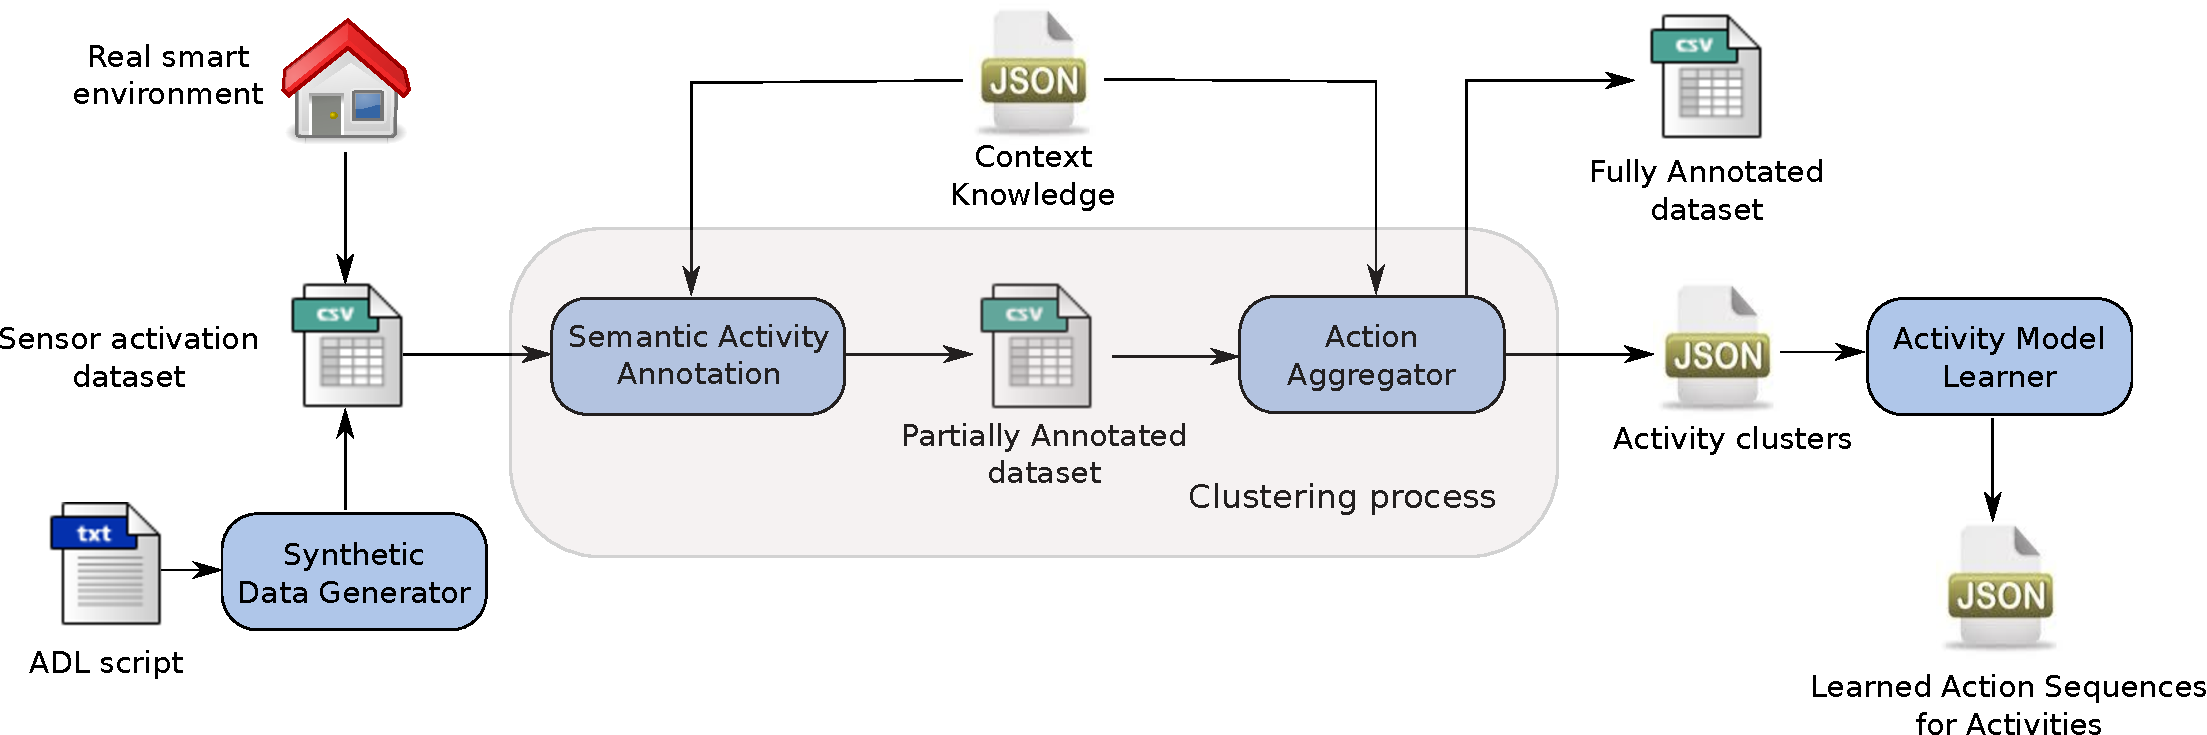
\includegraphics[width=\textwidth]{our_approach.pdf}
    \caption{The detailed design architecture of the proposed approach.}
    \label{fig-design}
\end{figure}

\subsection{Semantic Activity Annotation ($SA^3$)}
\label{subsec-sa3}
The $SA^3$ algorithm is used as the initialisation step of a clustering process. As explained in \cite{Azkune2014}, it uses IAMs to run a specially designed pattern recognition algorithm, where IAMs act as the patterns to be recognised. The algorithm is shown to work with positive sensor noise (sensors that are activated when they should not), missing sensor noise (sensors that are not activated when they should) and varied order of actions (the order in which actions are executed does not influence the performance of $SA^3$).

In this paper, a new feature has been added to the $SA^3$ algorithm described in \cite{Azkune2014}: activity location inference. Let $S=\{a, b, c, d\}$ be a sequence of actions, where $a$ and $d$ pertain to the IAM of activity $A$. For location inference, only actions that pertain to the IAM of the detected activity are considered, since all the other actions of the sequence $S$ cannot be considered as part of the activity yet. For instance, some of those actions might be produced by positive noise. Hence, the sequence $S$ is an activity $A$ with location $L$ \textit{iff} $a$ and $d$ have been executed in the same location and that location is compatible with $A$ activity's locations. As an example, assume actions \textit{hasBook} and \textit{useFurniture} pertain to the IAM of \textit{ReadBook}. Assume also that \textit{hasBook} action has been mapped from \textit{book-a} object and \textit{useFurniture} action from \textit{sofa} object. \textit{ReadBook} can be performed in the lounge or in the bedroom, according to context knowledge, but not in both. As \textit{book-a} object is in the bedroom but \textit{sofa} object is in the lounge, the sequence containing \textit{hasBook(book-a)} and \textit{useFurniture(sofa)} cannot form an activity. Activity location inference has shown to decrease $SA^3$ algorithm's false positive rates considerably.

The result of $SA^3$ is a sensor activation dataset named \textit{partially annotated dataset}, where actions describing an activity are labelled with that activity name. All the other actions will be labelled with the special label \textit{None}. We call the resulting file \textit{partially annotated} because actions that do not pertain to the IAMs of detected activities are not treated yet. 